\documentclass{jlreq}

% 日本語フォント
\usepackage[haranoaji]{luatexja-preset}

% abstract環境（jlreq デフォルトで定義済み）

% 基本パッケージ
\usepackage{geometry}
\usepackage{setspace}
\usepackage{fancyhdr}

% 数式
\usepackage{amsmath,amssymb,amsthm}
\usepackage{mathtools}

% 図表
\usepackage{graphicx}
\usepackage{svg}
\usepackage{float}
\usepackage{booktabs}
\usepackage{array}
\usepackage{longtable}
\usepackage{tikz}
\usepackage{pgfplots}
\pgfplotsset{compat=1.18}
\usetikzlibrary{arrows.meta,positioning,shapes}

% 参考文献
\usepackage[backend=biber,style=numeric,sorting=none]{biblatex}
\addbibresource{references.bib}

% リンク・URL
\usepackage[colorlinks=true,linkcolor=blue,citecolor=red,urlcolor=blue]{hyperref}
\usepackage{url}

% その他
\usepackage{enumerate}
\usepackage{enumitem}
% caption: ltjsbookと競合するため読み込み不要
%\usepackage{caption}
%\usepackage{subcaption}
\usepackage{listings}
\usepackage{xcolor}

% ページ設定
\geometry{top=25mm, bottom=25mm, left=25mm, right=25mm, footskip=10mm, headheight=17pt}

% 行間設定
\onehalfspacing

% ヘッダー・フッター
\pagestyle{fancy}
\fancyhf{}
\fancyhead[L]{\leftmark}
\fancyfoot[C]{\thepage}

% コードリスティング設定
\lstset{
  basicstyle=\ttfamily\small,
  keywordstyle=\color{blue},
  commentstyle=\color{green!60!black},
  stringstyle=\color{red},
  numbers=left,
  numberstyle=\tiny\color{gray},
  frame=single,
  breaklines=true,
  showstringspaces=false
}

% 定理環境
\newtheorem{theorem}{定理}
\newtheorem{lemma}{補題}
\newtheorem{definition}{定義}
\newtheorem{proposition}{命題}

% タイトル情報
\title{タイトル}
\author{著者名}
\date{\today}

\begin{document}

\maketitle

\begin{abstract}
  概要を記す.
\end{abstract}

\tableofcontents
\newpage

% 章ごとのファイルを読み込む
\section{はじめに}

\subsection{研究背景}

研究の背景などを書く.


\subsection{研究目的}

本稿の目的は以下の通りである:

\section{背景と関連研究}

\subsection{研究の背景}

本研究の背景について述べる.

\subsection{ネットワーク構造}

図\ref{fig:network}にネットワークの例を示す.

\begin{figure}[H]
  \centering
  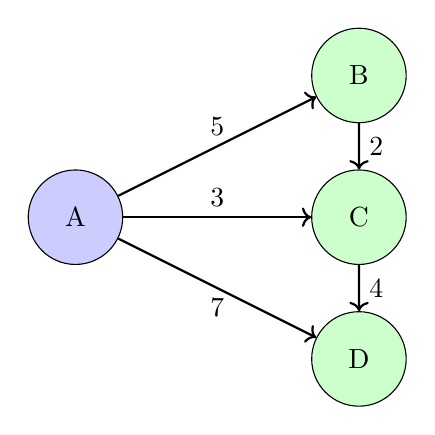
\begin{tikzpicture}[scale=1.2]
  % ノードA
  \node[circle, draw, fill=blue!20, minimum size=1.2cm] (A) at (0,0) {A};
  
  % ノードB, C, D
  \node[circle, draw, fill=green!20, minimum size=1.2cm] (B) at (3,1.5) {B};
  \node[circle, draw, fill=green!20, minimum size=1.2cm] (C) at (3,0) {C};
  \node[circle, draw, fill=green!20, minimum size=1.2cm] (D) at (3,-1.5) {D};
  
  % エッジ
  \draw[->, thick] (A) -- (B) node[midway, above] {5};
  \draw[->, thick] (A) -- (C) node[midway, above] {3};
  \draw[->, thick] (A) -- (D) node[midway, below] {7};
  
  \draw[->, thick] (B) -- (C) node[midway, right] {2};
  \draw[->, thick] (C) -- (D) node[midway, right] {4};
\end{tikzpicture}

  \caption{ネットワーク構造の例}
  \label{fig:network}
\end{figure}


\section{手法と実験}

\subsection{データ分析}

データの分析例を図\ref{fig:scatter}に示す.

\begin{figure}[H]
  \centering
  \begin{tikzpicture}[scale=1.0]
  % 座標軸
  \draw[->] (-0.5,0) -- (5,0) node[right] {$x$};
  \draw[->] (0,-0.5) -- (0,4) node[above] {$y$};
  
  % グリッド
  \draw[gray!30, thin] (0,0) grid (4.5,3.5);
  
  % データポイント
  \fill[blue] (1,1) circle (3pt);
  \fill[blue] (2,1.8) circle (3pt);
  \fill[blue] (3,2.5) circle (3pt);
  \fill[blue] (4,3.2) circle (3pt);
  
  % 近似直線
  \draw[red, thick, dashed] (0.5,0.5) -- (4.5,3.5);
  
  % ラベル
  \node[blue] at (4.2,3.5) {データ};
  \node[red] at (3.5,2.5) {近似線};
\end{tikzpicture}

  \caption{データの散布と近似線}
  \label{fig:scatter}
\end{figure}

\subsection{関数の比較}

複数の関数の比較を図\ref{fig:functions}に示す.

\begin{figure}[H]
  \centering
  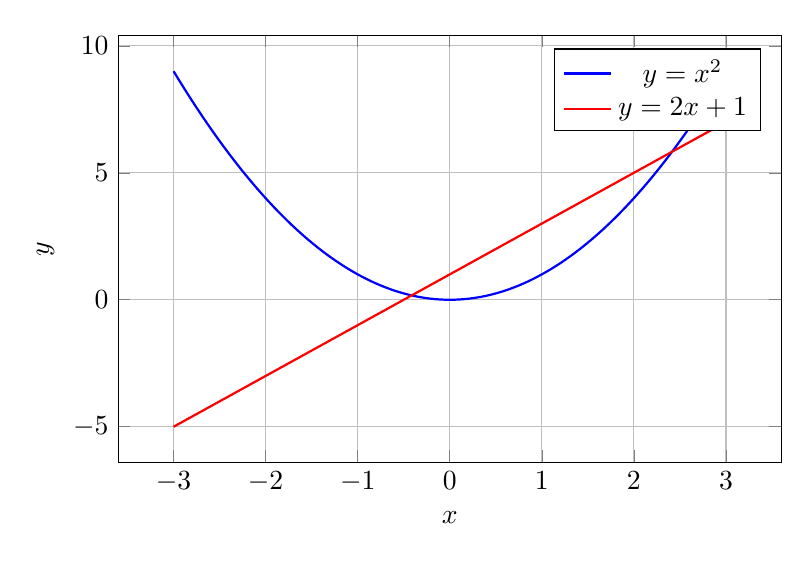
\begin{tikzpicture}
  \begin{axis}[
    xlabel={$x$},
    ylabel={$y$},
    grid=major,
    width=10cm,
    height=7cm,
    legend pos=north east
  ]
  \addplot[blue, thick, domain=-3:3, samples=100] {x^2};
  \addplot[red, thick, domain=-3:3, samples=100] {2*x+1};
  \legend{$y=x^2$, $y=2x+1$}
  \end{axis}
\end{tikzpicture}

  \caption{関数のプロット例}
  \label{fig:functions}
\end{figure}



\section{結論}

ここに結論を記す

\subsection{今後の課題}

今後の課題を記す

\section*{謝辞}
本研究の議論にあたり有益な助言をいただいた関係者各位に感謝申し上げます.

\nocite{*}
\printbibliography[title=参考文献]

\end{document}
